\chapter{Supernova Remnants} \label{appendix:snrs}

A SNR is the expanding remains %(kinetic energy and cosmic rays)
after a supernova event. SNRs have long been proposed as a site for cosmic-ray acceleration \citep{1934CoMtW...3...73B}. In this section I will briefly describe the evolution of SNRs.

\begin{SCfigure}[0.5][hbtp]
    \centering
    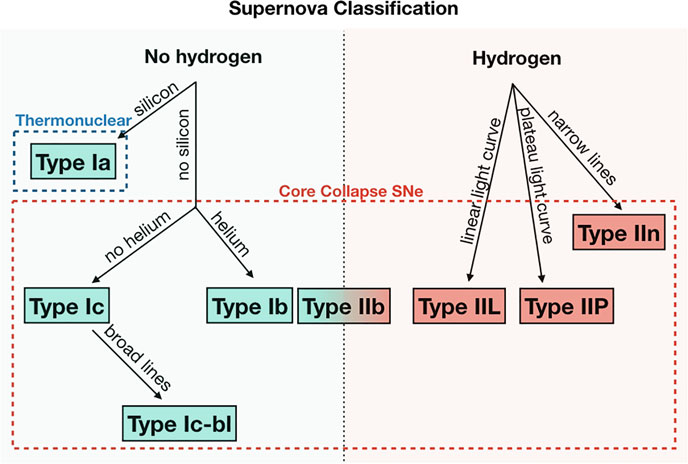
\includegraphics[width=0.8\textwidth]{A1_Supernova_Remnants/Images/supernova_classification.pdf}
    \caption{Supernovae are historically categorised into different classifications based on their absorption line and light curves. Image courtesy of \cite{alma9928040781501811}.}
    \label{fig:A1_supernova_classification}
\end{SCfigure}


\section{The Supernova}

Approximately two to three supernovae occur in the Milky Way per century \citep{1984AuJPh..37..321M,1994ApJS...92..487T}. Supernova are historically classified based on their light curves (a plot of the source's intensity vs time) and absorption lines. Type I supernovae tend to have no hydrogen absorption lines and light curves rapidly peak ($\approx 1-2$ days) and then slowly decay \citep{alma9928040781501811}. In contrast, Hydrogen absorption lines are observed in Type II supernovae and do not have as high a maximum in their light curves as Type I supernova \citep{alma9928040781501811}. Type I and II supernova can be further subdivided based on the appearance of silicon or helium absorption lines and the shape of their light curve.
\newpar
White dwarves are the remnant of stars whose mass was not sufficient to form a neutron star or black hole. As stars are typically born in groups, the white dwarf can accrete matter from its companion. This companion is normally another white dwarf or star. Once the mass of the white dwarf exceeds the Chandrasekhar limit ($1.4~M_\odot$), electron degeneracy pressure cannot withhold gravitational collapse and the star goes supernova. Supernovae with white dwarves as their progenitor are known as Type Ia supernova. A star with enough mass ($\gtrsim 8~M_\odot$) undergo core collapse to form a neutron star or black hole. These type of supernova tend to form Type Ib, Type Ic and Type II supernovae. See \autoref{fig:A1_supernova_classification} for further classification of supernovae based on their absorption lines and light cuves.

\section{Stages of a Supernova Remnant}

\begin{wrapfigure}[16]{R}{0.41\textwidth}
	    \centering
	    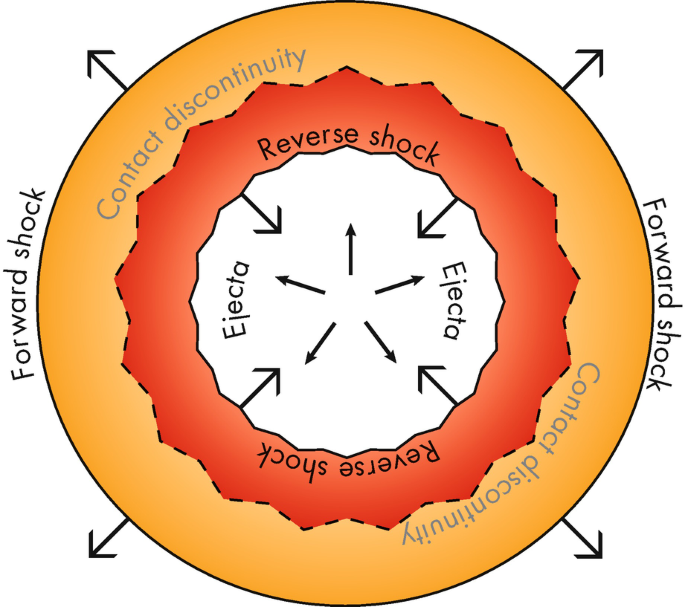
\includegraphics[width=0.4\textwidth]{A1_Supernova_Remnants/Images/SNR_evolution.png}
	    \caption{Illustration of the forward and reverse shocks of a SNR in its Sedov-Taylor phase of its evolution. Image courtesy of \cite{alma9928040781501811}}
	    \label{fig:A1_SNR_Evolution}
\end{wrapfigure}

A supernova releases around $10^{53}\,\ergs$ of energy, with $99\%$ of this energy being channelled into high-energy neutrinos. The remaining $10^{51}\,\ergs$ mostly goes into kinetic energy. Approximately $10$ to $20\%$ of the kinetic energy ($10^{50}\,\ergs$) is transferred into accelerating cosmic rays \citep{2012SSRv..173..369H}. The supernova ejects material into the ISM at supersonic speeds (up to $10\%$ the speed of light). The interaction of ejected material with the ISM forms a shock wave ahead of the material which, in turn, creates a shell of plasma \citep{alma9928040781501811}. The evolution of the SNR can be divided into four stages:

\subsection{Free Expansion Phase}

Also classified as the ejecta-dominated phase, this phase occurs when the ejected mass from the supernova outweighs the mass of the swept up ISM ($M_\text{ej}>M_\text{sw}$) and can last for hundreds of years up to a thousand years after the initial supernova \citep{2008ARA&A..46...89R}. A supernova with kinetic energy $E$ ejects material with speed \citep{2022arXiv221102217B}:

\begin{equation}
    \begin{aligned}
        v&=\sqrt{\frac{2E}{M_\text{ej}}}\approx 10^4\quad\qty[\kmpersec]\text{ .} 
    \end{aligned}
\end{equation}

The outermost shell interacts with the ISM forming a shock wave (forward shock) and a shell of `shocked' plasma which radiatively cools and decelerates  \citep{1972ARA&A..10..129W}. The ejecta behind this shell is now moving faster than the shocked plasma shell and collides, forming a reverse shock which propagates inwards relative to the forward shock. SNRs in the free expansion phase tend to be bright in X-rays due to synchrotron emission from high-energy electrons. An example of a SNR in its expansion phase is \mbox{G1.9+0.3} with an age of  $\approx 100\,\si{yr}$ and situated close to the Galactic centre. \citep{2008ApJ...680L..41R}

\subsection{Sedov-Taylor Phase}

When the swept up material outweighs the mass of the ejected material ($M_\text{sw}>M_\text{ej}$), the Sedov-Taylor (aka energy-conservation phase) begins. Radiative losses (through thermal and synchrotron radiation) are negligible and the SNR remnant expands adiabatically with radius and velocity \citep{alma9947651801811}:

\begin{equation}
    \begin{aligned}
        R &\propto t^{\frac{2}{5}} \\
        V&\propto t^{-\frac{3}{5}}\text{ .} 
    \end{aligned} \label{eq:A1_SNR_radius_velocity}
\end{equation}
Diffusive shock acceleration (see \autoref{sec:A2_finite_difference}) is believed to accelerate cosmic rays up to $\TeV$ energies. These cosmic rays escape the SNR and interact with the surrounding ISM via proton-proton interactions (\autoref{sec:chapter1_hadronic_gr_emission}) to produce gamma-rays. SNRs in their Sedov-Taylor phase are still bright in X-rays through synchrotron radiation and last up to $\approx 20\,\kiloyear$. Cassiopeia A is an example of a SNR entering its Sedov-Taylor phase \citep{1999ApJS..120..299T}.

\subsection{Snow-Plough Phase}

Expansion of the SNR slows down as the system ages (see \autoref{eq:A1_SNR_radius_velocity}). When the shock velocity reaches $200\,\kmpersec$ and temperatures are below $10^6\,\si{K}$, ionised atoms (e.g. hydrogen) recombine with free electrons and emit electromagnetic radiation in the radio-optical spectrum \citep{1972ARA&A..10..129W}.  This is known as the Snow-Plough phase where the expansion is governed by the conservation of momentum rather than energy \citep{alma9928040781501811,}. The age at which a SNR is estimated to reach its snow plough phase is given by:

\begin{equation}
    \begin{aligned}
    t_\text{SP}&=446 \qty(\frac{E_{51}}{n_H\,\si{\per\centi\meter\cubed}})^\frac{1}{3}\text{ ,} 
    \end{aligned}
\end{equation}
\noindent where $n$ is the density of the ambient medium \citep{alma9928040781501811,}. An SNR in its Snow-Plough phase expands in a rate $R\propto t^{1/4}$ \citep{1972ARA&A..10..129W}. The SNR associated with \mbox{HESS J1825-137} is believed to be entering the Snow-Plough phase based on the characteristic age of the associated pulsar and observed H$\alpha$ lines \citep{2016MNRAS.458.2813V}.

\subsubsection{Merging with the Interstellar Medium}

The SNR expansion velocity continues to slow down until it reaches the speed of sound in the ISM and the SNR dissipates ($\approx 10\,\kmpersec$) \citep{1972ARA&A..10..129W}. SNRs tend to have a life time approximately $1$ million years.

